\documentclass[10pt, a4paper]{article}\usepackage[]{graphicx}\usepackage[]{xcolor}
% maxwidth is the original width if it is less than linewidth
% otherwise use linewidth (to make sure the graphics do not exceed the margin)
\makeatletter
\def\maxwidth{ %
  \ifdim\Gin@nat@width>\linewidth
    \linewidth
  \else
    \Gin@nat@width
  \fi
}
\makeatother

\definecolor{fgcolor}{rgb}{0.345, 0.345, 0.345}
\newcommand{\hlnum}[1]{\textcolor[rgb]{0.686,0.059,0.569}{#1}}%
\newcommand{\hlstr}[1]{\textcolor[rgb]{0.192,0.494,0.8}{#1}}%
\newcommand{\hlcom}[1]{\textcolor[rgb]{0.678,0.584,0.686}{\textit{#1}}}%
\newcommand{\hlopt}[1]{\textcolor[rgb]{0,0,0}{#1}}%
\newcommand{\hlstd}[1]{\textcolor[rgb]{0.345,0.345,0.345}{#1}}%
\newcommand{\hlkwa}[1]{\textcolor[rgb]{0.161,0.373,0.58}{\textbf{#1}}}%
\newcommand{\hlkwb}[1]{\textcolor[rgb]{0.69,0.353,0.396}{#1}}%
\newcommand{\hlkwc}[1]{\textcolor[rgb]{0.333,0.667,0.333}{#1}}%
\newcommand{\hlkwd}[1]{\textcolor[rgb]{0.737,0.353,0.396}{\textbf{#1}}}%
\let\hlipl\hlkwb

\usepackage{framed}
\makeatletter
\newenvironment{kframe}{%
 \def\at@end@of@kframe{}%
 \ifinner\ifhmode%
  \def\at@end@of@kframe{\end{minipage}}%
  \begin{minipage}{\columnwidth}%
 \fi\fi%
 \def\FrameCommand##1{\hskip\@totalleftmargin \hskip-\fboxsep
 \colorbox{shadecolor}{##1}\hskip-\fboxsep
     % There is no \\@totalrightmargin, so:
     \hskip-\linewidth \hskip-\@totalleftmargin \hskip\columnwidth}%
 \MakeFramed {\advance\hsize-\width
   \@totalleftmargin\z@ \linewidth\hsize
   \@setminipage}}%
 {\par\unskip\endMakeFramed%
 \at@end@of@kframe}
\makeatother

\definecolor{shadecolor}{rgb}{.97, .97, .97}
\definecolor{messagecolor}{rgb}{0, 0, 0}
\definecolor{warningcolor}{rgb}{1, 0, 1}
\definecolor{errorcolor}{rgb}{1, 0, 0}
\newenvironment{knitrout}{}{} % an empty environment to be redefined in TeX

\usepackage{alltt}

%%%%%%%%%%%%%%%%%%%%%%%%%%%%%%%%%%%%%%%%%%%%%%%%%%%%%%%%%%%%%%%%

\usepackage[OT4]{polski}
\usepackage[utf8]{inputenc}
\usepackage[top=2.5cm, bottom=2.5cm, left=2cm, right=2cm]{geometry}
\usepackage{graphicx}
\usepackage{float}
\usepackage{amsmath}
\usepackage[colorlinks=true, linkcolor=blue]{hyperref}
\newtheorem{wn}{Wniosek}


%%%%%%%%%%%%%%%%%%%%%%%%%%%%%%%%%%%%%%%%%%%%%%%%%%%%%%%%%%%%%%%%



\IfFileExists{upquote.sty}{\usepackage{upquote}}{}
\begin{document}




%%%%%%%%%%%%%%%%%%%%%%%%%%%%%%%%%%%%%%%%%%%%%%%%%%%%%%%%%%%%%%%%

\title{Symulacyjna analiza własności rozkładów asymptotycznych i testowanie białoszumowości}
\author{Stanisław Olek}
\maketitle
\tableofcontents

\section{Symulacyjna analiza własności rozkładów asymptotycznych}

Przeprowadzimy symulacyjną analizę własności rozkładów asymptotycznych estymatorów dla szeregów czasowych typu biały szum. Analizowane będą następujące estymatory:

\begin{enumerate}
  \item Estymator wartości oczekiwanej $\mu$ - średnia próbkowa:
  \begin{equation}
  \bar{X}_n=\frac{1}{n}\sum_{t=1}^n X_t
  \label{eq:srednia}
  \end{equation}
  
  \item Estymator funkcji autokowariancji $\gamma(h)$:
  \begin{equation}
  \hat{\gamma}(h)=\frac{1}{n}\sum_{t=1}^{n-h}(X_{t+h}-\bar{X}_n)(X_t-\bar{X}_n), \quad \text{dla } h=0,1,\ldots,n-1
  \label{eq:autokowariancja}
  \end{equation}
  
\end{enumerate}


\subsection{Estymator wartości oczekiwanej $\mu$}
Najpierw zbadamy własności rozkładu estymatora wartości oczekiwanej $\mu$ zdefiniowanego w równaniu \eqref{eq:srednia}, czyli średniej próbkowej, dla różnych rozkładów i różnych długości szeregów $n$. Analiza zostanie przeprowadzona dla trzech rozkładów: normalnego, wykładniczego oraz jednostajnego.

\newpage
\subsubsection{Rozkład normalny}


\begin{knitrout}
\definecolor{shadecolor}{rgb}{0.969, 0.969, 0.969}\color{fgcolor}\begin{figure}[H]

{\centering 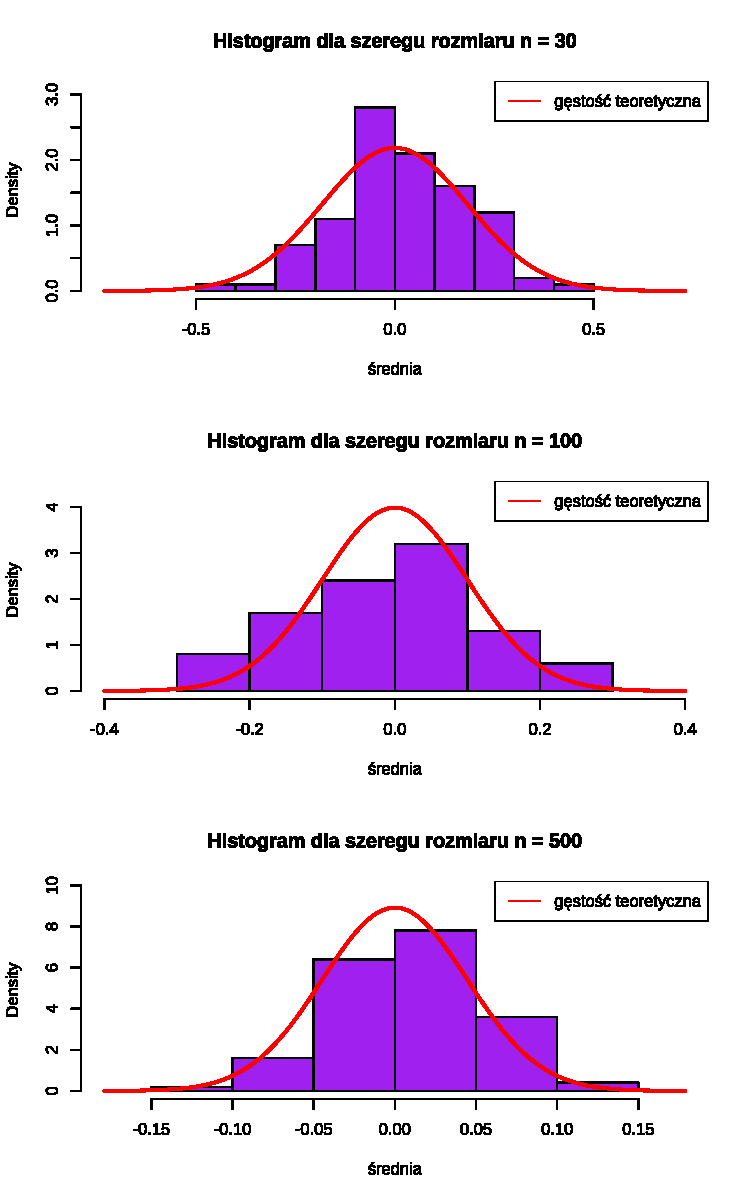
\includegraphics[width=\maxwidth]{figure/analiza-sredniej-norm-hist-1} 

}

\caption[Histogramy dla estymatora średniej dla różnych długości szeregów $n$ z rozkładu normalnego]{Histogramy dla estymatora średniej dla różnych długości szeregów $n$ z rozkładu normalnego}\label{fig:analiza-sredniej-norm-hist}
\end{figure}

\end{knitrout}


\begin{knitrout}
\definecolor{shadecolor}{rgb}{0.969, 0.969, 0.969}\color{fgcolor}\begin{figure}[H]

{\centering 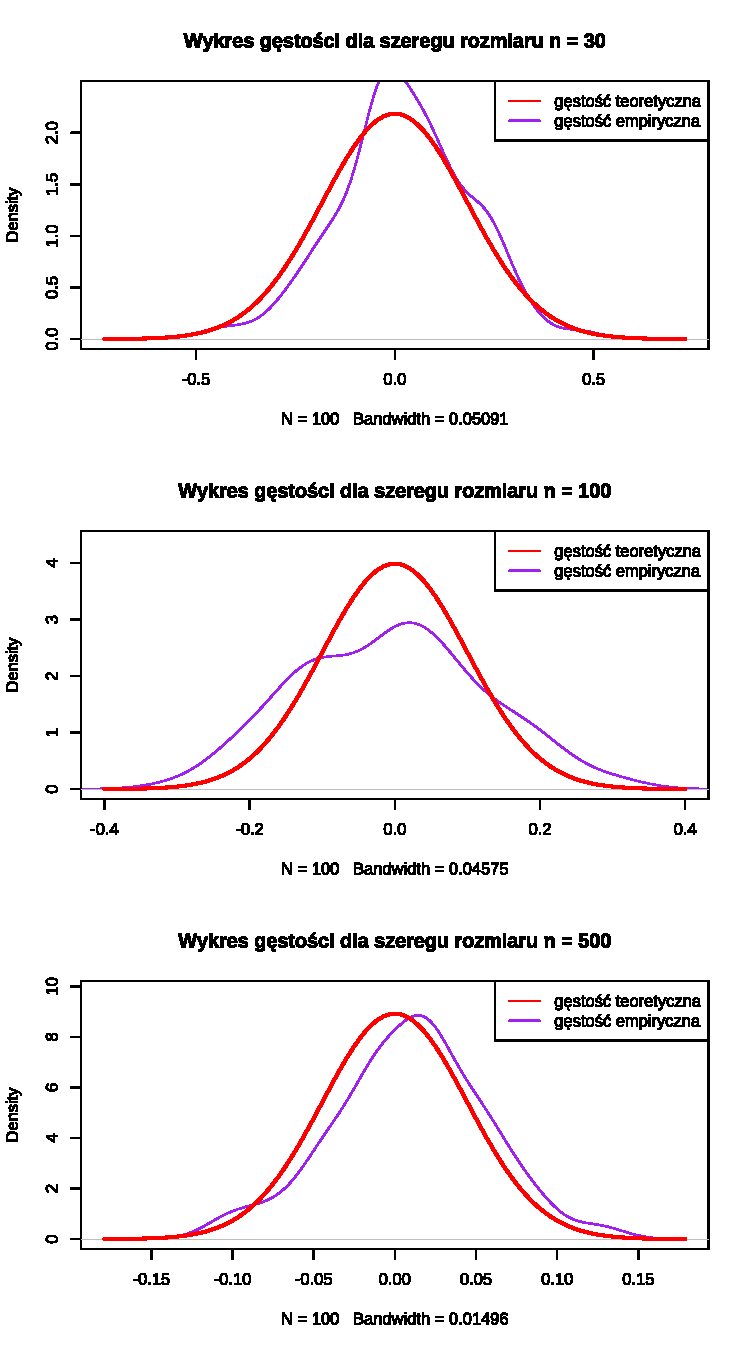
\includegraphics[width=\maxwidth]{figure/analiza-sredniej-norm-dens-1} 

}

\caption[Wykresy gęstości dla estymatora średniej dla różnych długości szeregów $n$ z rozkładu normalnego]{Wykresy gęstości dla estymatora średniej dla różnych długości szeregów $n$ z rozkładu normalnego}\label{fig:analiza-sredniej-norm-dens}
\end{figure}

\end{knitrout}



\begin{knitrout}
\definecolor{shadecolor}{rgb}{0.969, 0.969, 0.969}\color{fgcolor}\begin{figure}[H]

{\centering 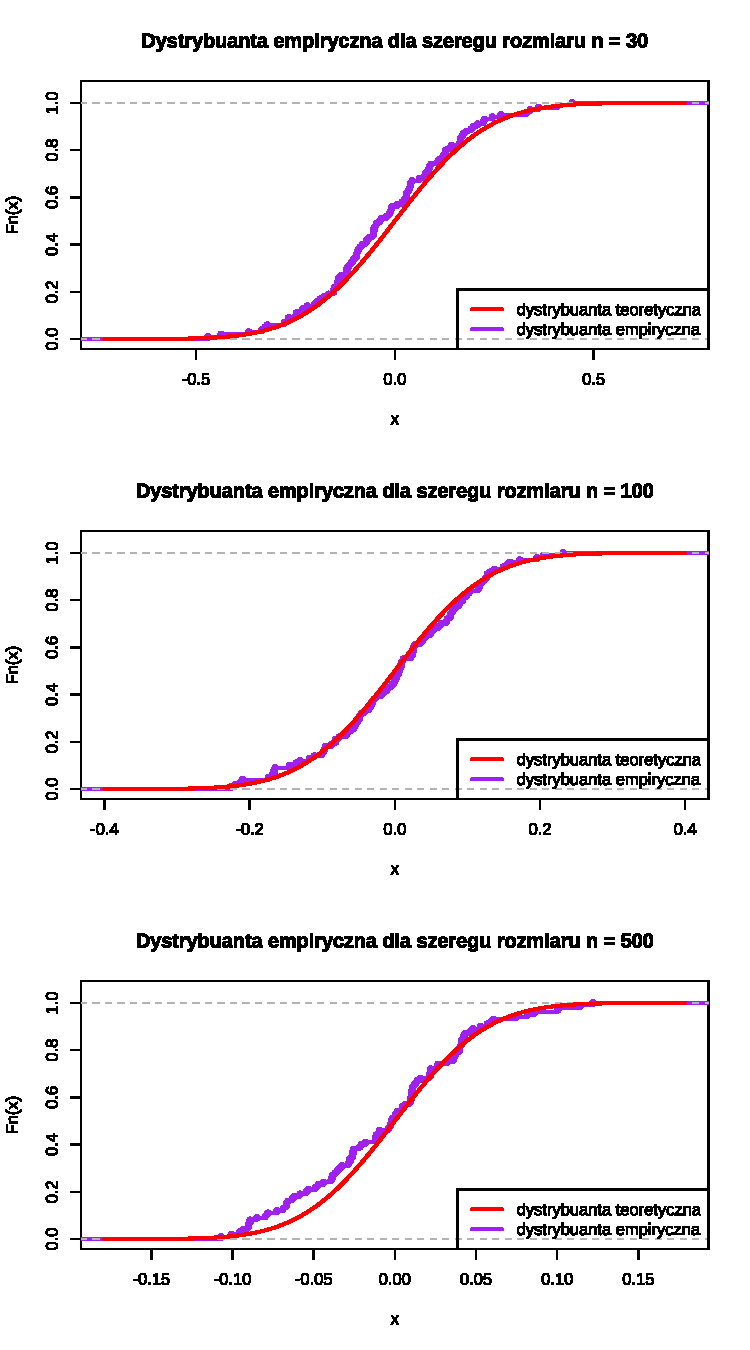
\includegraphics[width=\maxwidth]{figure/analiza-sredniej-norm-dystr-emp-1} 

}

\caption[Dystrybuanty empiryczne dla estymatora średniej dla różnych długości szeregów $n$ z rozkładu normalnego]{Dystrybuanty empiryczne dla estymatora średniej dla różnych długości szeregów $n$ z rozkładu normalnego}\label{fig:analiza-sredniej-norm-dystr-emp}
\end{figure}

\end{knitrout}


\begin{knitrout}
\definecolor{shadecolor}{rgb}{0.969, 0.969, 0.969}\color{fgcolor}\begin{figure}[H]

{\centering 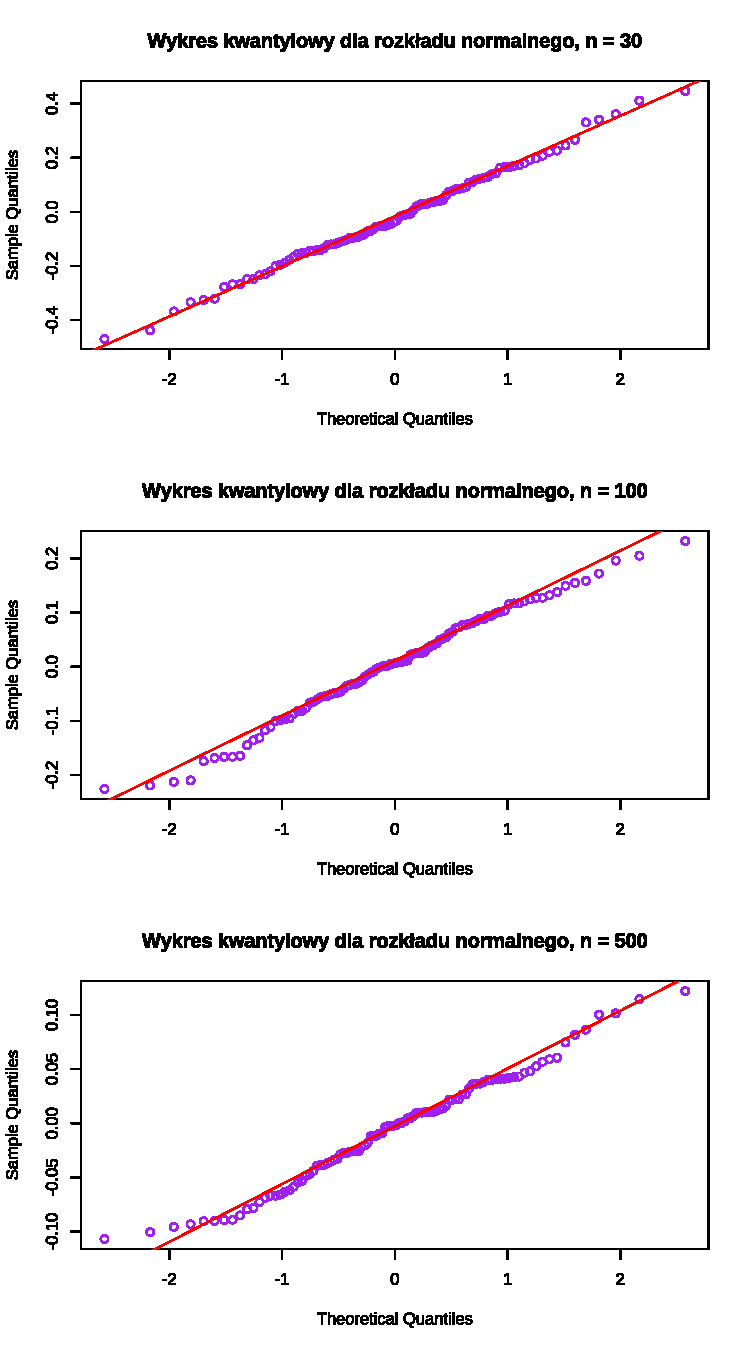
\includegraphics[width=\maxwidth]{figure/analiza-srednie-wykresy-kwant-1} 

}

\caption[Wykresy kwantylowe dla estymatora średniej dla różnych długości szeregów $n$ z rozkładu normalnego]{Wykresy kwantylowe dla estymatora średniej dla różnych długości szeregów $n$ z rozkładu normalnego}\label{fig:analiza-srednie-wykresy-kwant}
\end{figure}

\end{knitrout}


Analiza estymatora średniej próbkowej dla danych z rozkładu normalnego wykazała następujące własności:

\begin{itemize}
    \item Dla wszystkich analizowanych długości szeregów ($n = 30, 100, 500$) rozkład empiryczny średniej próbkowej wykazał idealne dopasowanie do teoretycznego rozkładu normalnego, co potwierdzają:
        \begin{itemize}
            \item Symetryczny kształt histogramów ze skupieniem wokół wartości 0 jak widać na [\ref{fig:analiza-sredniej-norm-hist}]
            \item Nakładanie się empirycznych i teoretycznych krzywych gęstości jak widać na [\ref{fig:analiza-sredniej-norm-dens}]
            \item Niemal całkowite pokrywanie się dystrybuant empirycznych z teoretyczną dystrybuantą normalną jak widać na [\ref{fig:analiza-sredniej-norm-dystr-emp}]
            \item Punkty na wykresach kwantylowych układają się wzdłuż linii teoretycznej jak widać na [\ref{fig:analiza-srednie-wykresy-kwant}]
        \end{itemize}
      
      \item Nawet dla małych prób ($n = 30$) brak obserwowalnych odchyleń od normalności
\end{itemize}

%%%%%%%%%%%%%%%%%%%%%%%%%%%%%%%%%%%%%%%%%%%%%%%%%%%%%%%%%%%%%%%%

\newpage
\subsubsection{Rozkład wykładniczy $Exp(1)$}


\begin{knitrout}
\definecolor{shadecolor}{rgb}{0.969, 0.969, 0.969}\color{fgcolor}\begin{figure}[H]

{\centering 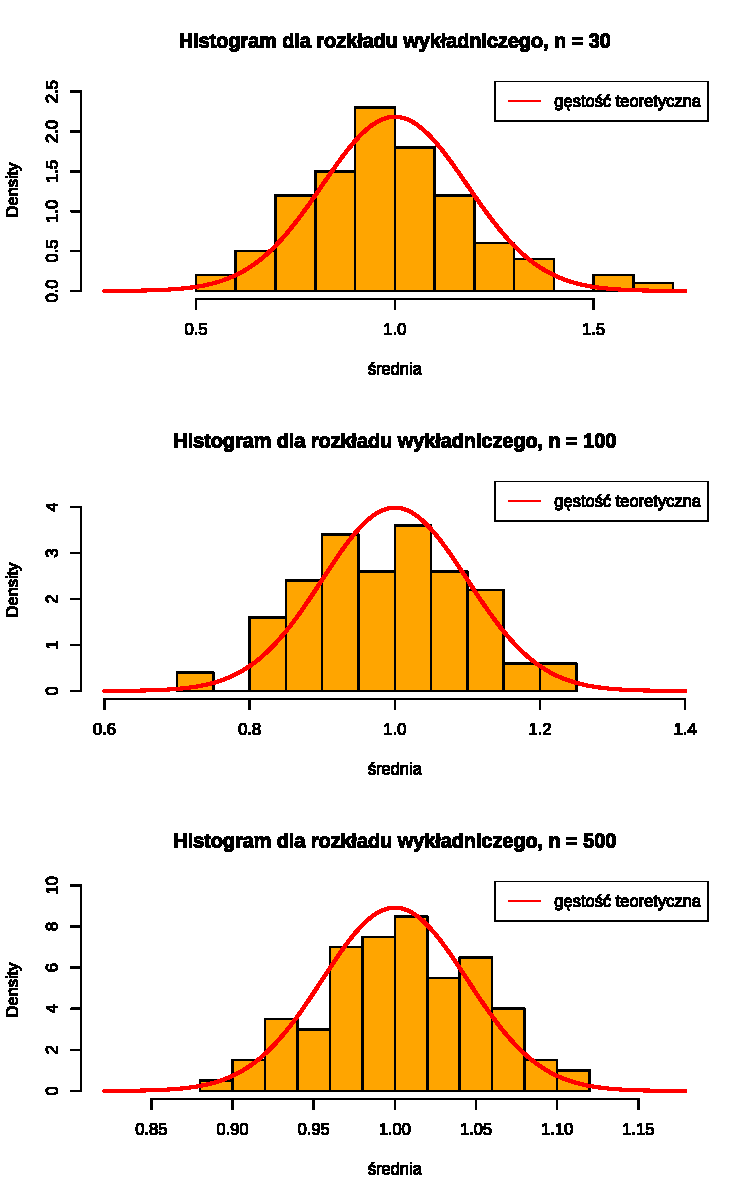
\includegraphics[width=\maxwidth]{figure/analiza-sredniej-exp-hist-1} 

}

\caption[Histogramy dla estymatora średniej dla różnych długości szeregów $n$ z rozkładu wykładniczego]{Histogramy dla estymatora średniej dla różnych długości szeregów $n$ z rozkładu wykładniczego}\label{fig:analiza-sredniej-exp-hist}
\end{figure}

\end{knitrout}

\begin{knitrout}
\definecolor{shadecolor}{rgb}{0.969, 0.969, 0.969}\color{fgcolor}\begin{figure}[H]

{\centering 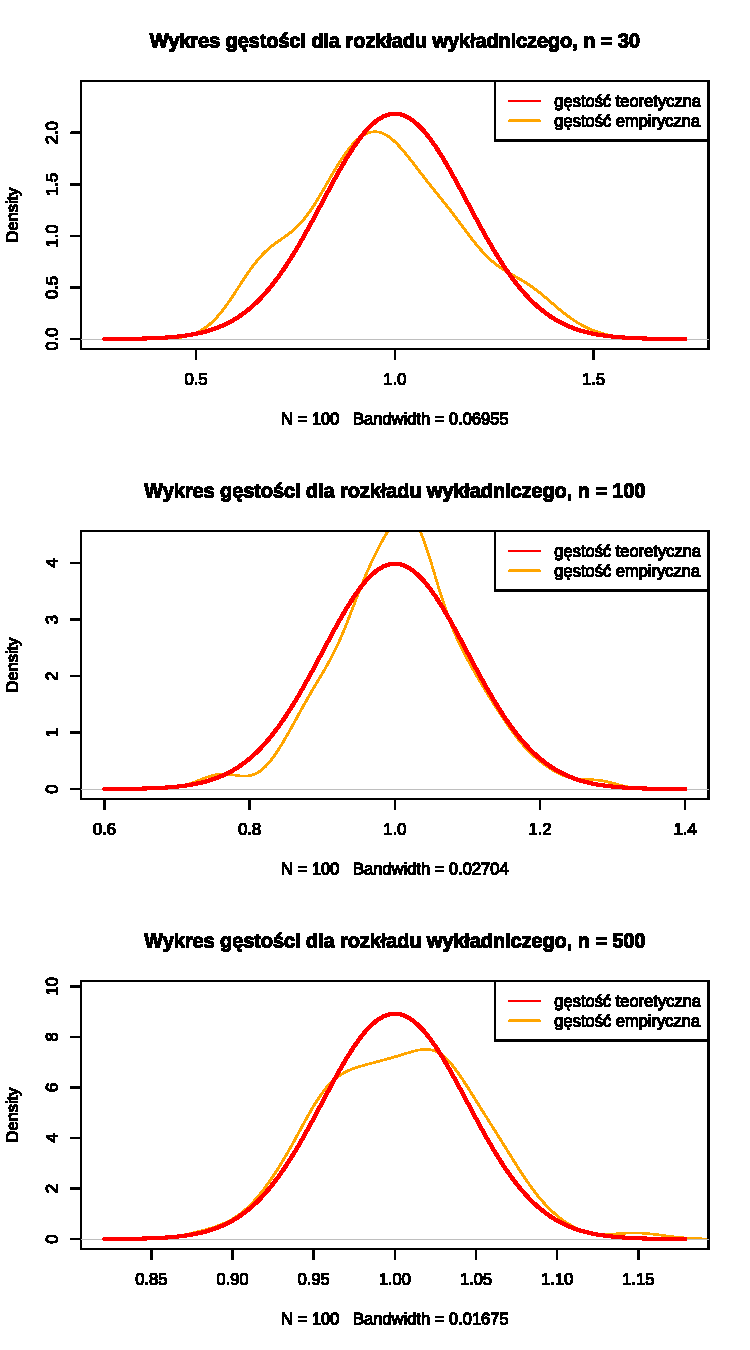
\includegraphics[width=\maxwidth]{figure/analiza-sredniej-exp-dens-1} 

}

\caption[Wykresy gęstości dla estymatora średniej dla różnych długości szeregów $n$ z rozkładu wykładniczego]{Wykresy gęstości dla estymatora średniej dla różnych długości szeregów $n$ z rozkładu wykładniczego}\label{fig:analiza-sredniej-exp-dens}
\end{figure}

\end{knitrout}

\begin{knitrout}
\definecolor{shadecolor}{rgb}{0.969, 0.969, 0.969}\color{fgcolor}\begin{figure}[H]

{\centering 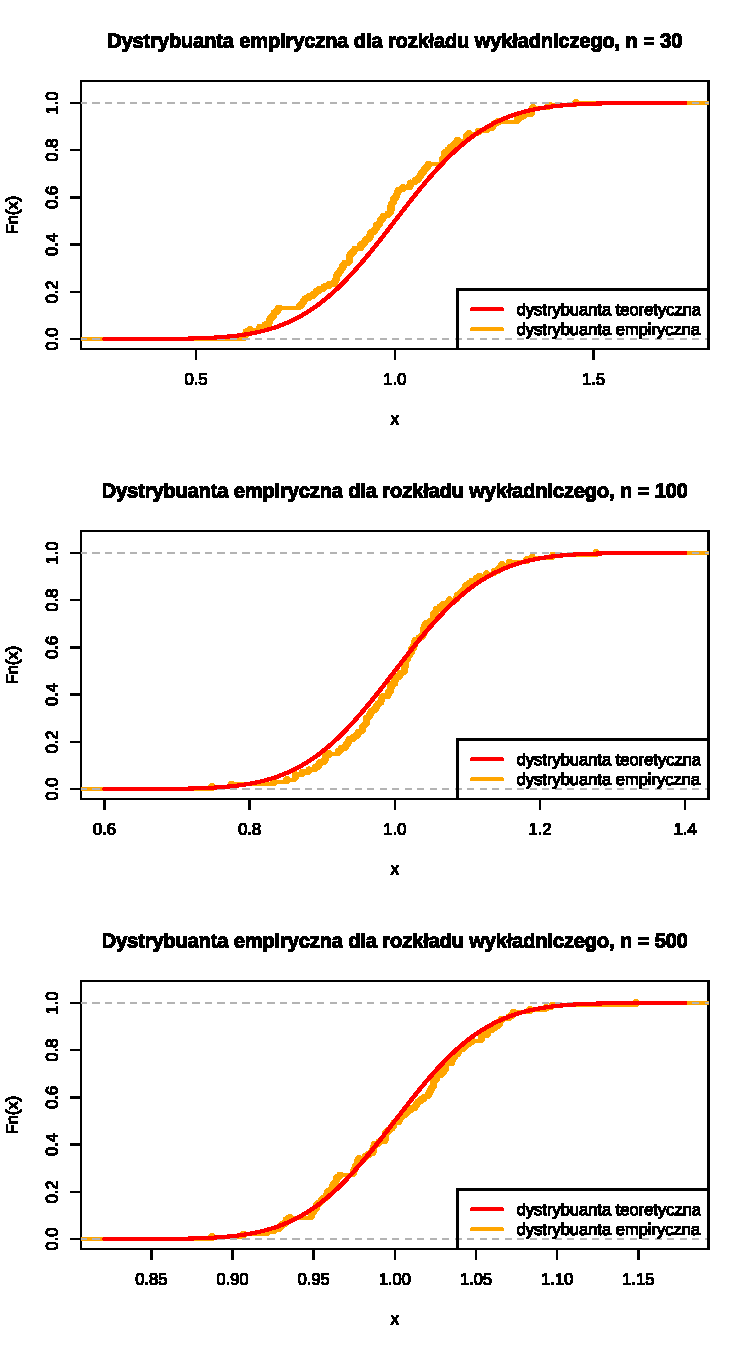
\includegraphics[width=\maxwidth]{figure/analiza-sredniej-exp-dystr-emp-1} 

}

\caption[Dystrybuanty empiryczne dla estymatora średniej dla różnych długości szeregów $n$ z rozkładu wykładniczego]{Dystrybuanty empiryczne dla estymatora średniej dla różnych długości szeregów $n$ z rozkładu wykładniczego}\label{fig:analiza-sredniej-exp-dystr-emp}
\end{figure}

\end{knitrout}


\begin{knitrout}
\definecolor{shadecolor}{rgb}{0.969, 0.969, 0.969}\color{fgcolor}\begin{figure}[H]

{\centering 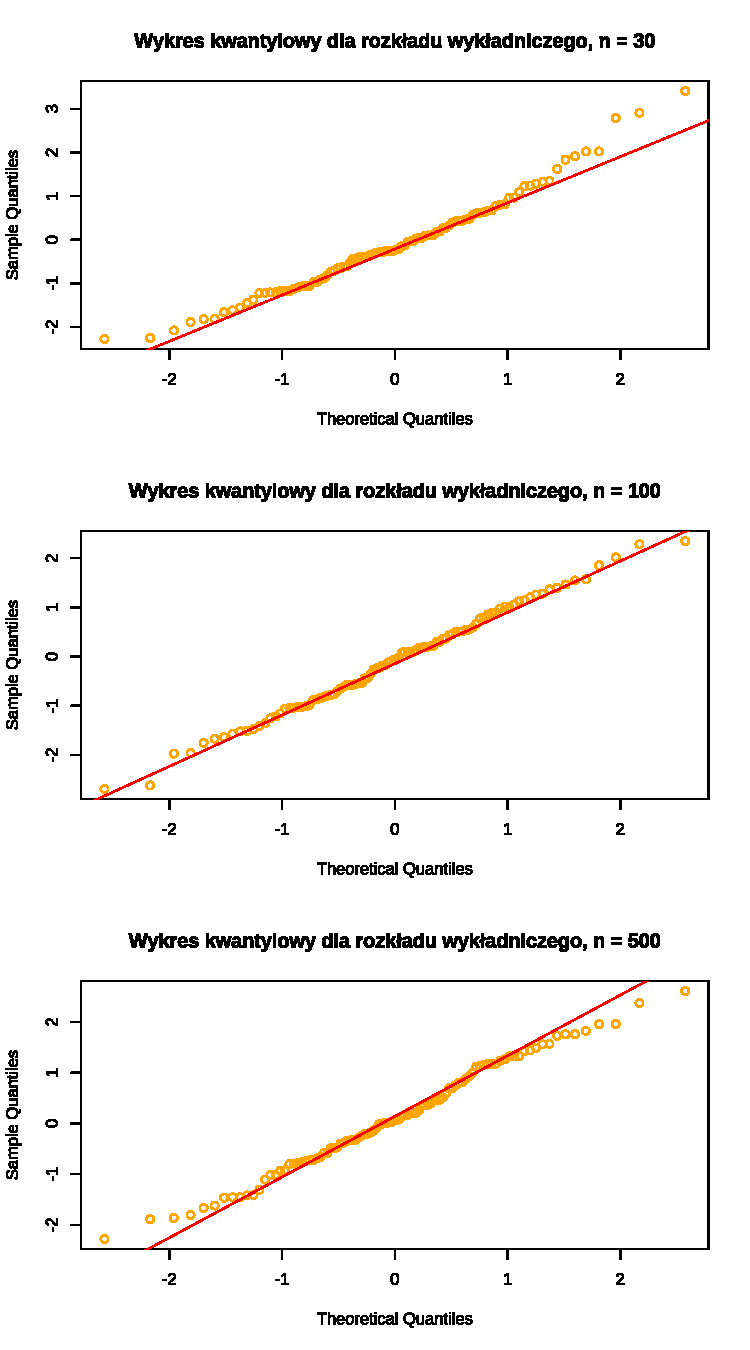
\includegraphics[width=\maxwidth]{figure/analiza-srednie-exp-wykresy-kwant-1} 

}

\caption[Wykresy kwantylowe dla estymatora średniej dla różnych długości szeregów $n$ z rozkładu wykładniczego]{Wykresy kwantylowe dla estymatora średniej dla różnych długości szeregów $n$ z rozkładu wykładniczego}\label{fig:analiza-srednie-exp-wykresy-kwant}
\end{figure}

\end{knitrout}

Analiza wyników dla rozkładu wykładniczego pokazuje właściwości asymptotyczne estymatora średniej. Obserwujemy, że:

\begin{itemize}
  \item Dla najmniejszej wielkości próby $n=30$ rozkład empiryczny estymatora wykazuje lekką asymetrię, co widać zarówno na histogramach [\ref{fig:analiza-sredniej-exp-hist}] jak i wykresach gęstości [\ref{fig:analiza-sredniej-exp-dens}]
  \item Wraz ze wzrostem rozmiaru próbki ($n=100$ i $n=500$) asymetria zanika, a rozkład empiryczny coraz lepiej przybliża rozkład normalny
  \item Dystrybuanty empiryczne [\ref{fig:analiza-sredniej-exp-dystr-emp}] pokazują wyraźne zbliżanie się do dystrybuanty rozkładu normalnego $N(1, 1/\sqrt{n})$ gdy $n$ rośnie. Dla $n=500$ dopasowanie jest niemal idealne
  \item Wykresy kwantylowe [\ref{fig:analiza-srednie-exp-wykresy-kwant}] potwierdzają normalność rozkładu dla większych $n$, choć nawet przy $n=500$ można zauważyć niewielkie odchylenia w ogonach rozkładu
\end{itemize}

Obserwacje te potwierdzają teoretyczne przewidywania, według którego średnia próbkowa zmiennych niezależnych o rozkładzie wykładniczym będzie asymptotycznie zbiegać do rozkładu normalnego $N(1, 1/\sqrt{n})$, gdzie $1$ jest wartością oczekiwaną rozkładu wykładniczego $Exp(1)$.

%%%%%%%%%%%%%%%%%%%%%%%%%%%%%%%%%%%%%%%%%%%%%%%%%%%%%%%%%%%%%%%%

\newpage 
\subsubsection{Rozkład jednostajny $Unif[0,1]$}


\begin{knitrout}
\definecolor{shadecolor}{rgb}{0.969, 0.969, 0.969}\color{fgcolor}\begin{figure}[H]

{\centering 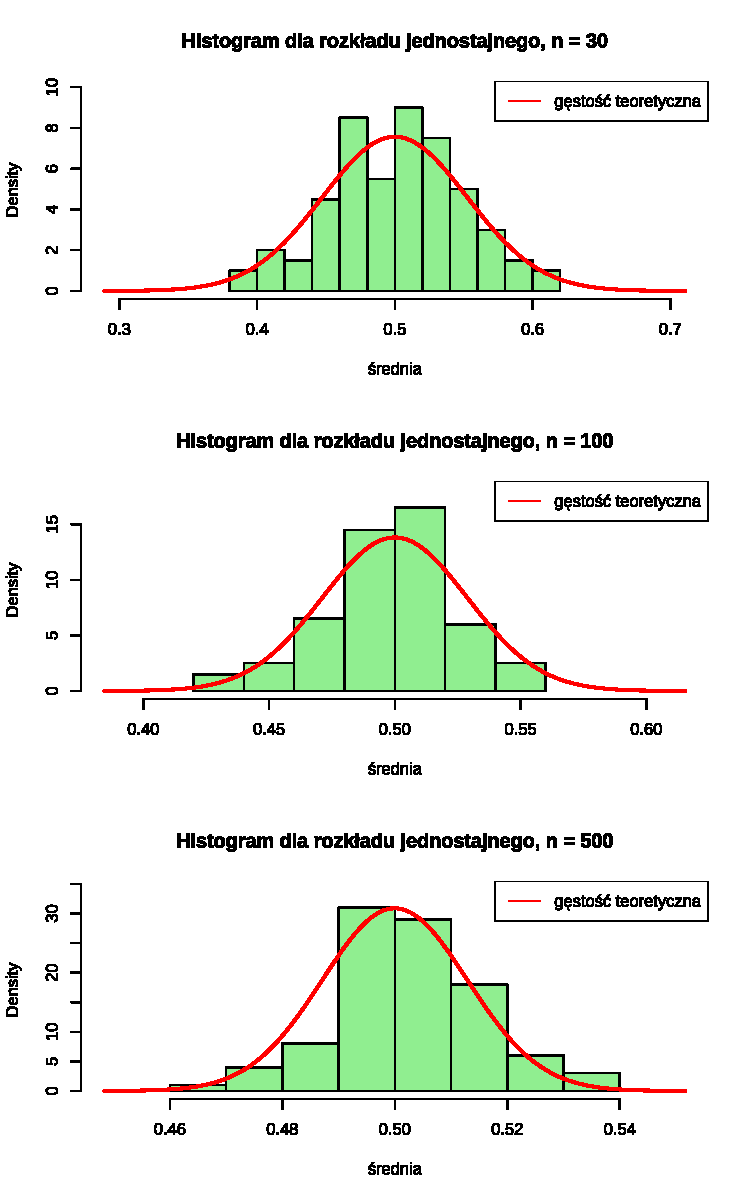
\includegraphics[width=\maxwidth]{figure/analiza-sredniej-unif-hist-1} 

}

\caption[Histogramy dla estymatora średniej dla różnych długości szeregów $n$ z rozkładu jednostajnego]{Histogramy dla estymatora średniej dla różnych długości szeregów $n$ z rozkładu jednostajnego}\label{fig:analiza-sredniej-unif-hist}
\end{figure}

\end{knitrout}

\begin{knitrout}
\definecolor{shadecolor}{rgb}{0.969, 0.969, 0.969}\color{fgcolor}\begin{figure}[H]

{\centering 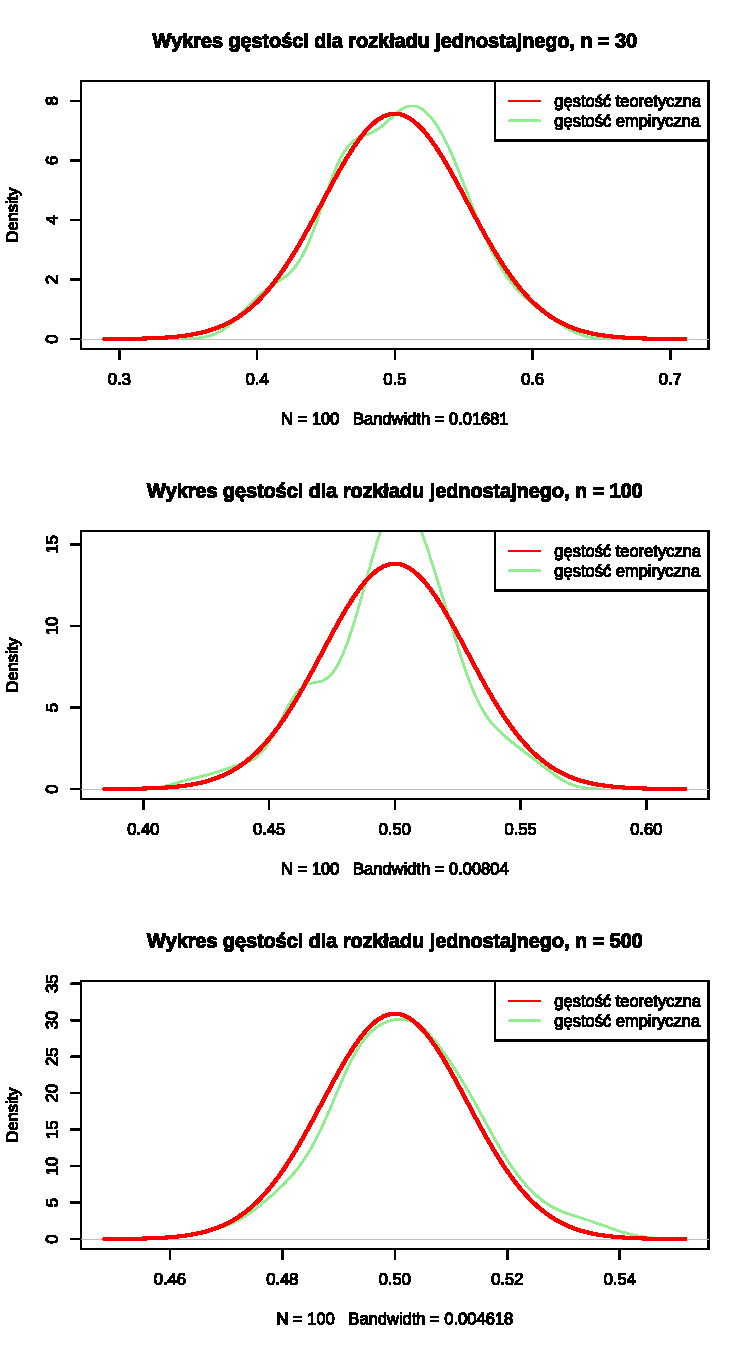
\includegraphics[width=\maxwidth]{figure/analiza-sredniej-unif-dens-1} 

}

\caption[Wykresy gęstości dla estymatora średniej dla różnych długości szeregów $n$ z rozkładu jednostajnego]{Wykresy gęstości dla estymatora średniej dla różnych długości szeregów $n$ z rozkładu jednostajnego}\label{fig:analiza-sredniej-unif-dens}
\end{figure}

\end{knitrout}

\begin{knitrout}
\definecolor{shadecolor}{rgb}{0.969, 0.969, 0.969}\color{fgcolor}\begin{figure}[H]

{\centering 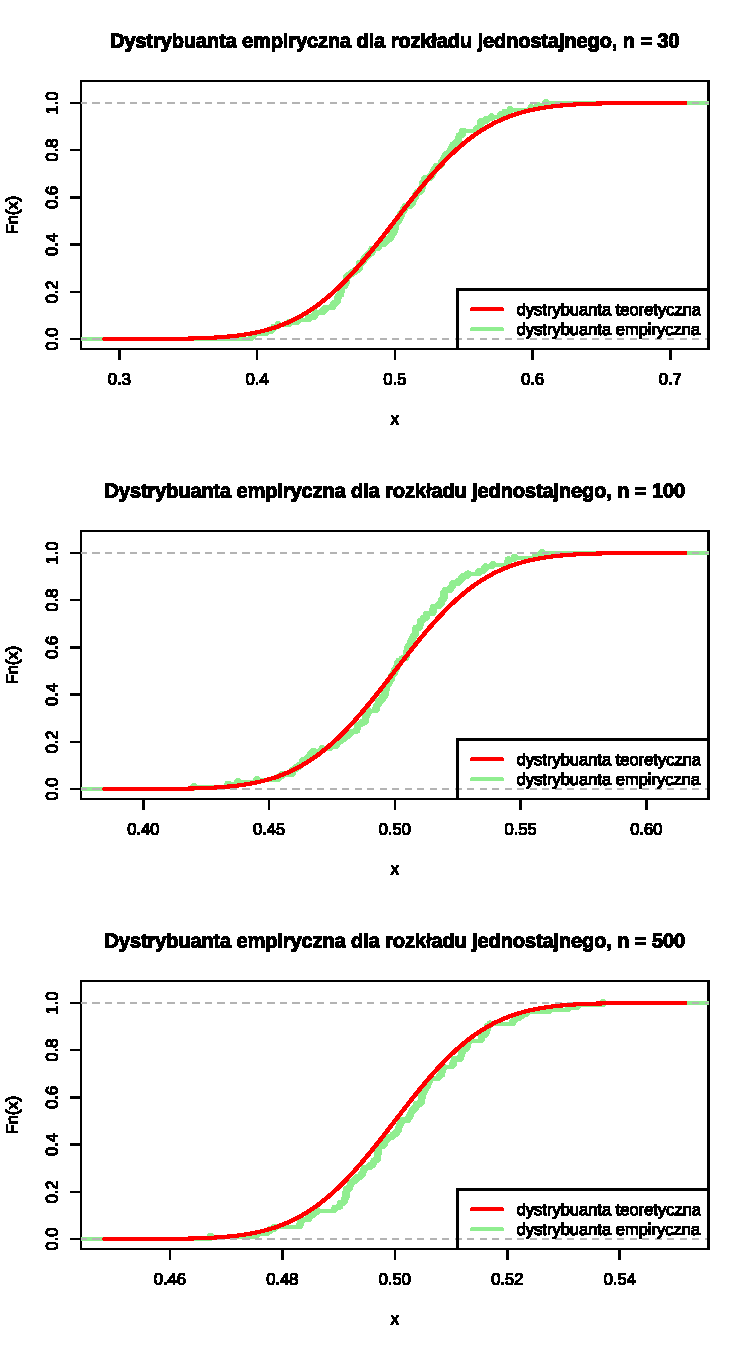
\includegraphics[width=\maxwidth]{figure/analiza-sredniej-unif-dystr-emp-1} 

}

\caption[Dystrybuanty empiryczne dla estymatora średniej dla różnych długości szeregów $n$ z rozkładu jednostajnego]{Dystrybuanty empiryczne dla estymatora średniej dla różnych długości szeregów $n$ z rozkładu jednostajnego}\label{fig:analiza-sredniej-unif-dystr-emp}
\end{figure}

\end{knitrout}

\begin{knitrout}
\definecolor{shadecolor}{rgb}{0.969, 0.969, 0.969}\color{fgcolor}\begin{figure}[H]

{\centering 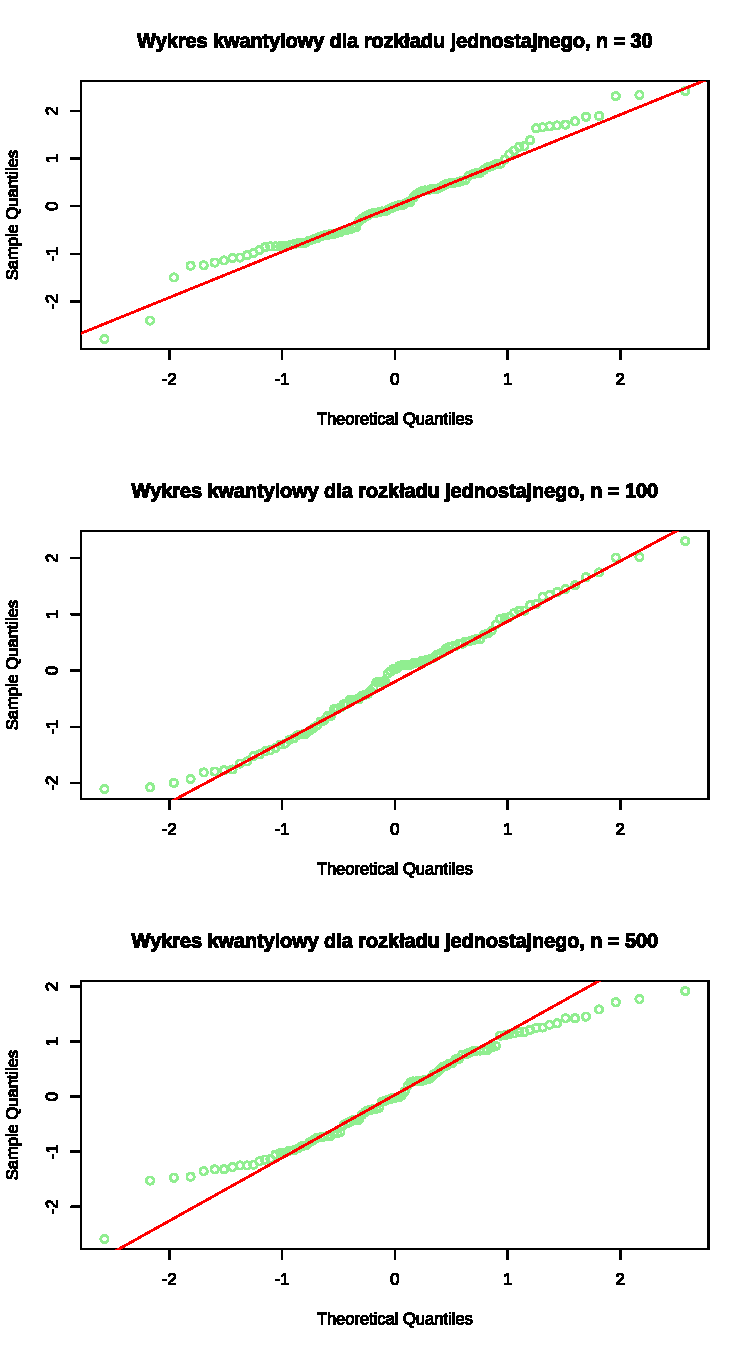
\includegraphics[width=\maxwidth]{figure/analiza-srednie-unif-wykresy-kwant-1} 

}

\caption[Wykresy kwantylowe dla estymatora średniej dla różnych długości szeregów $n$ z rozkładu jednostajnego]{Wykresy kwantylowe dla estymatora średniej dla różnych długości szeregów $n$ z rozkładu jednostajnego}\label{fig:analiza-srednie-unif-wykresy-kwant}
\end{figure}

\end{knitrout}


Na podstawie przeprowadzonej analizy estymatora średniej dla rozkładu jednostajnego $Unif[0,1]$ można sformułować następujące wnioski:

\begin{itemize}
    \item Wyniki symulacji potwierdzają, że rozkład średniej próbkowej z rozkładu jednostajnego dąży do rozkładu normalnego wraz ze wzrostem liczby obserwacji, jak widać na [\ref{fig:analiza-sredniej-unif-hist}]
    \item Wraz ze wzrostem liczności próby $n$ obserwujemy:
    \begin{itemize}
        \item Bardziej symetryczny kształt histogramu i rozkładu gęstości wokół wartości oczekiwanej $1/2$, jak widać na [\ref{fig:analiza-sredniej-unif-hist}]
        \item Coraz lepsze dopasowanie empirycznego rozkładu do teoretycznego rozkładu normalnego, jak widać na wykresach gęstości [\ref{fig:analiza-sredniej-unif-dens}]    
        \item Coraz lepsze dopasowanie do teoretycznej dystrybuanty rozkładu normalnego, jak widać na [\ref{fig:analiza-sredniej-unif-dystr-emp}]
        \item Punkty na wykresie kwantylowym układają się wzdłuż linii teoretycznej, co wskazuje na dobre dopasowanie do rozkładu normalnego, jak widać na [\ref{fig:analiza-srednie-unif-wykresy-kwant}]
        \end{itemize}
    \item Nawet dla stosunkowo małych liczności próby (np. $n = 30$), średnia próbkowa wykazuje już znaczną zbieżność do rozkładu normalnego
\end{itemize}





\subsection{Estymator funkcji autokowariancji $\gamma$}
Przeprowadzimy analizę własności estymatora autokowariancji zdefiniowanego w równaniu \eqref{eq:autokowariancja} dla różnych rozkładów białego szumu i długości szeregów.

\newpage
\subsubsection{Rozkład normalny}


\begin{knitrout}
\definecolor{shadecolor}{rgb}{0.969, 0.969, 0.969}\color{fgcolor}\begin{figure}[H]

{\centering 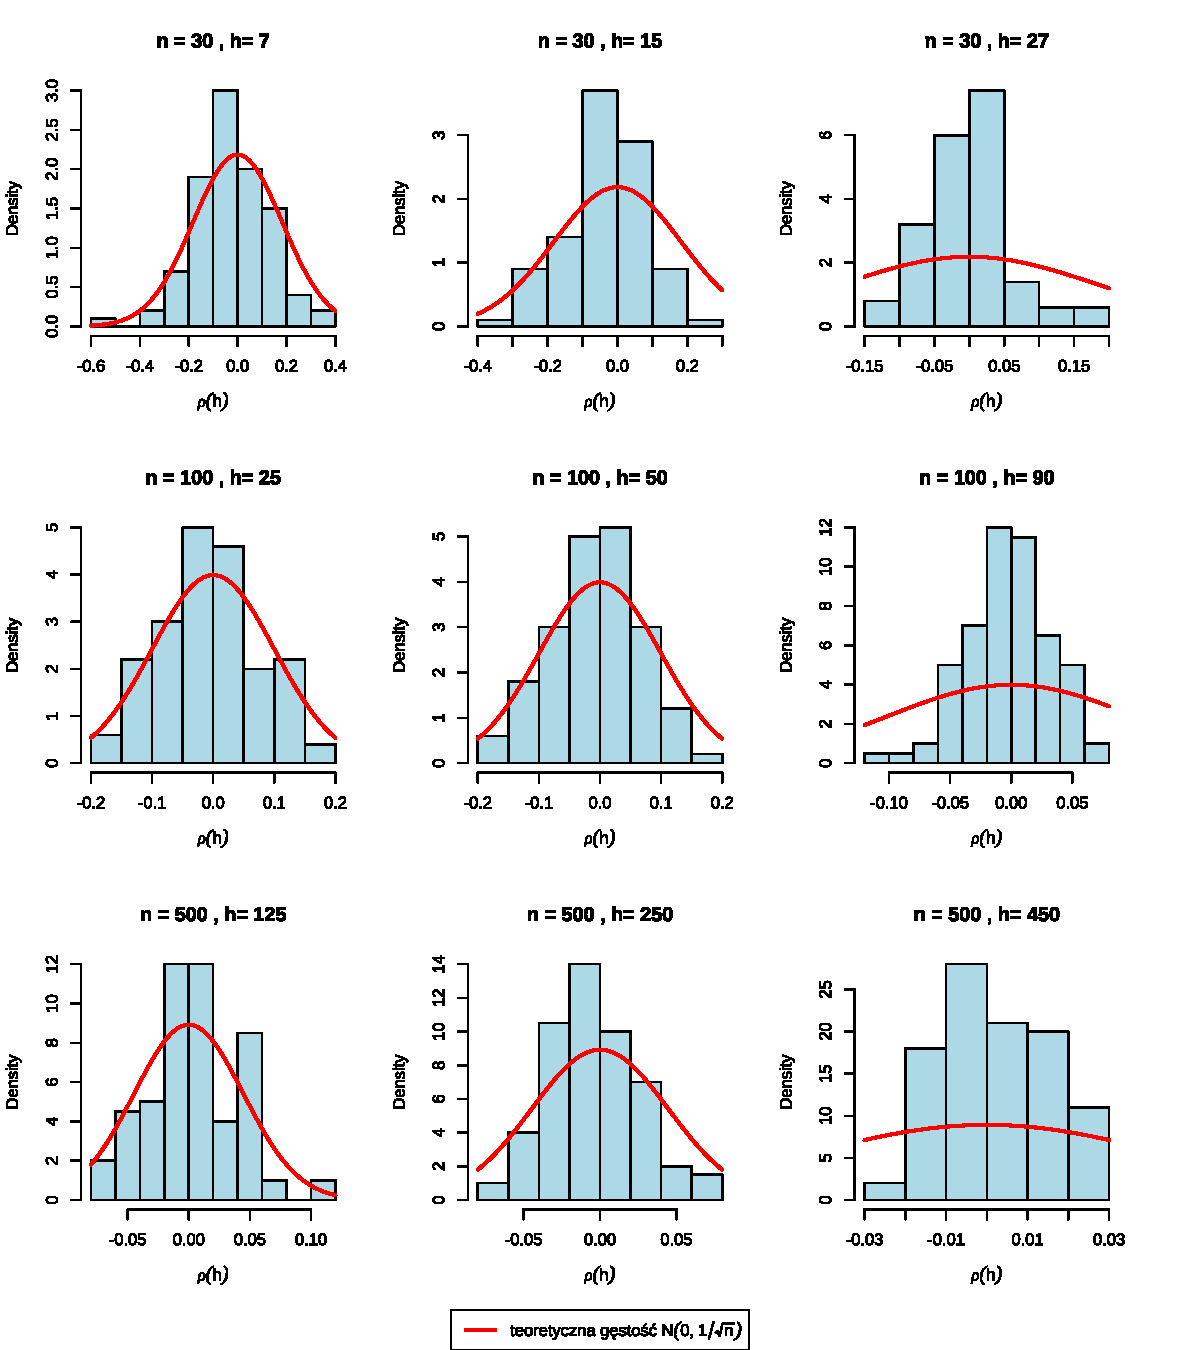
\includegraphics[width=\maxwidth]{figure/wykresy-gamma-norm-1} 

}

\caption[Histogramy dla estymatora funkcji autokowariancji dla różnych długości szeregów $n$ i różnych opóźnień $h$ z rozkładu normalnego]{Histogramy dla estymatora funkcji autokowariancji dla różnych długości szeregów $n$ i różnych opóźnień $h$ z rozkładu normalnego}\label{fig:wykresy-gamma-norm}
\end{figure}

\end{knitrout}


\newpage
Wyniki dla róźnych $n$ i opóźnień $h$ przedstawiono na [\ref{fig:wykresy-gamma-norm}].
Analiza estymatora funkcji autokowariancji dla danych z rozkładu normalnego wykazała następujące własności:

\begin{itemize}
\item Wpływ długości szeregu $n$:
  \begin{itemize}
  \item Wzrost $n$ zmniejsza wariancję estymatora
  \item Dla $n=500$ rozkład ściśle skupiony wokół 0
  \end{itemize}

\item Zachowanie dla dużych $h$:
  \begin{itemize}
  \item Przy $h \approx 0.9n$ wariancja wzrasta kilkukrotnie
  \item Pojawiają się wartości odstające i asymetria
  \end{itemize}
\end{itemize}


Estymator $\hat{\gamma}(h)$ jest asymptotycznie normalny $N(0,1/n)$, ale dla $h \approx n$ traci własności asymptotyczne.


\newpage
\subsubsection{Rozkład wykładniczy $Exp(1)$}


\begin{knitrout}
\definecolor{shadecolor}{rgb}{0.969, 0.969, 0.969}\color{fgcolor}\begin{figure}[H]

{\centering 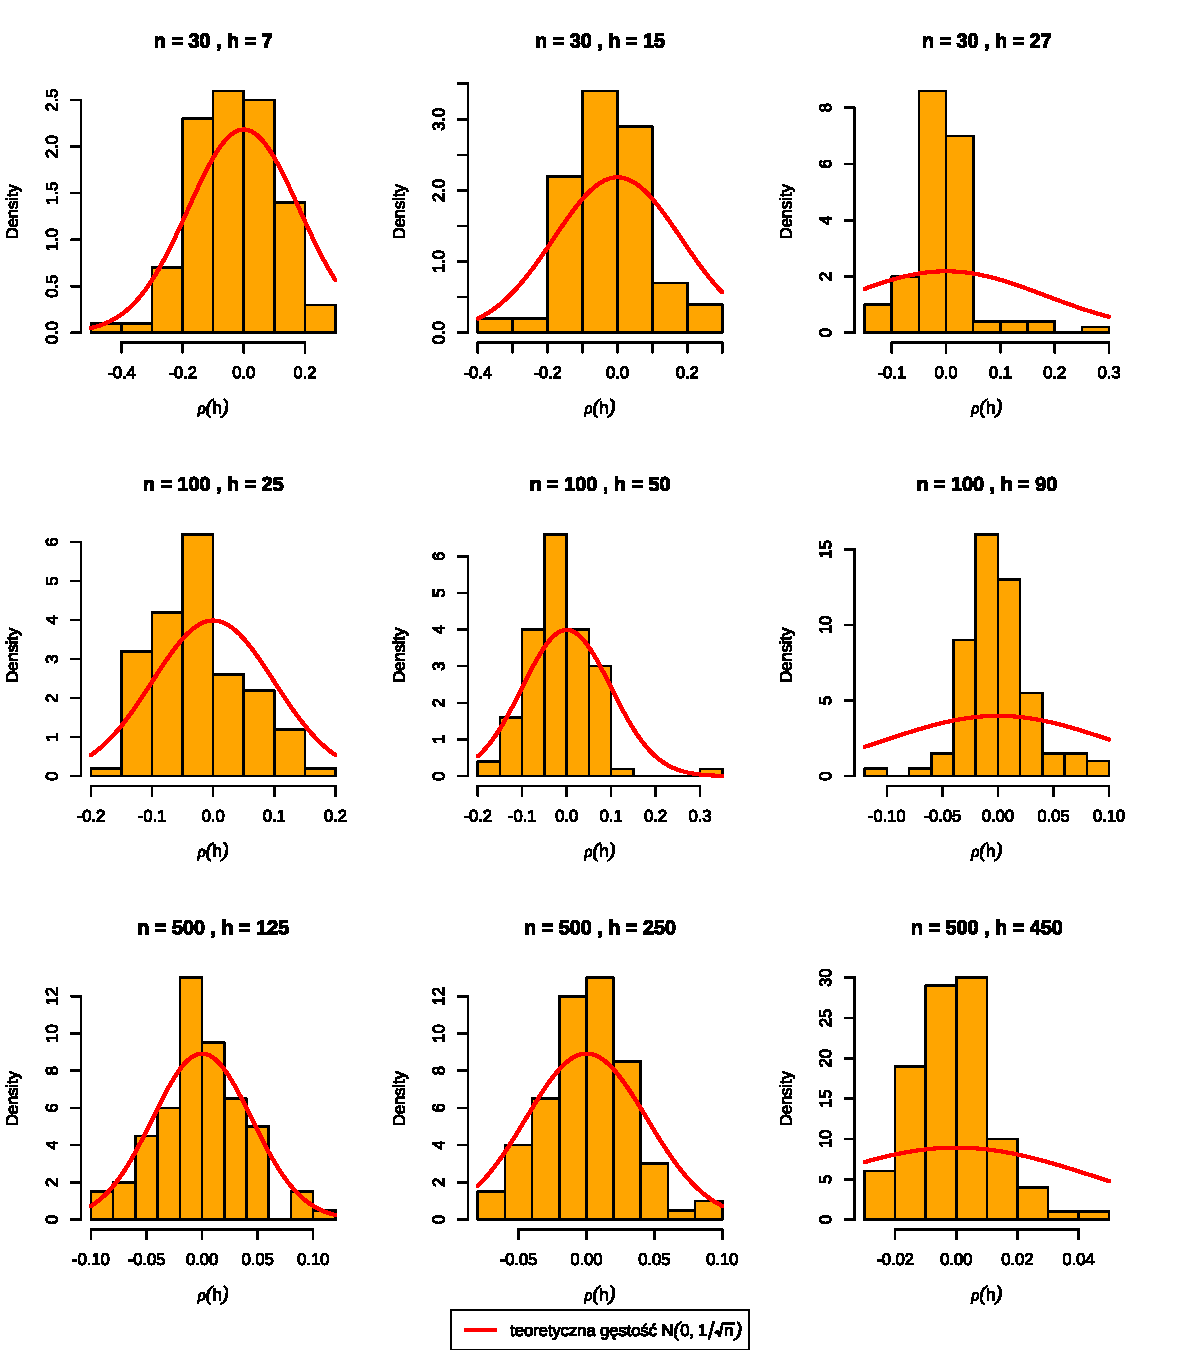
\includegraphics[width=\maxwidth]{figure/wykresy-gamma-exp-1} 

}

\caption[Histogramy dla estymatora funkcji autokowariancji dla różnych długości szeregów $n$ i różnych opóźnień $h$ z rozkładu wykładniczego]{Histogramy dla estymatora funkcji autokowariancji dla różnych długości szeregów $n$ i różnych opóźnień $h$ z rozkładu wykładniczego}\label{fig:wykresy-gamma-exp}
\end{figure}

\end{knitrout}

Wyniki dla róźnych $n$ i opóźnień $h$ przedstawiono na [\ref{fig:wykresy-gamma-exp}]. Analiza estymatora funkcji autokowariancji dla danych z rozkładu wykładniczego wykazała następujące własności:
  \begin{itemize}
  \item Dla $n=30$ widoczna asymetria rozkładu
  \item Dla $h \approx 0.9n$ większa skośność niż w rozkładzie normalnym
  \item Asymptotyczna normalność osiągana dopiero dla $n \geq 100$
\end{itemize}

Estymator $\hat{\gamma}(h)$ zachowuje własności asymptotyczne nawet dla silnie skośnych danych, ale wymaga większych próbek ($n \geq 100$) dla dobrej aproksymacji.


\subsubsection{Rozkład jednostajny $Unif[0,1]$}


\begin{knitrout}
\definecolor{shadecolor}{rgb}{0.969, 0.969, 0.969}\color{fgcolor}\begin{figure}[H]

{\centering 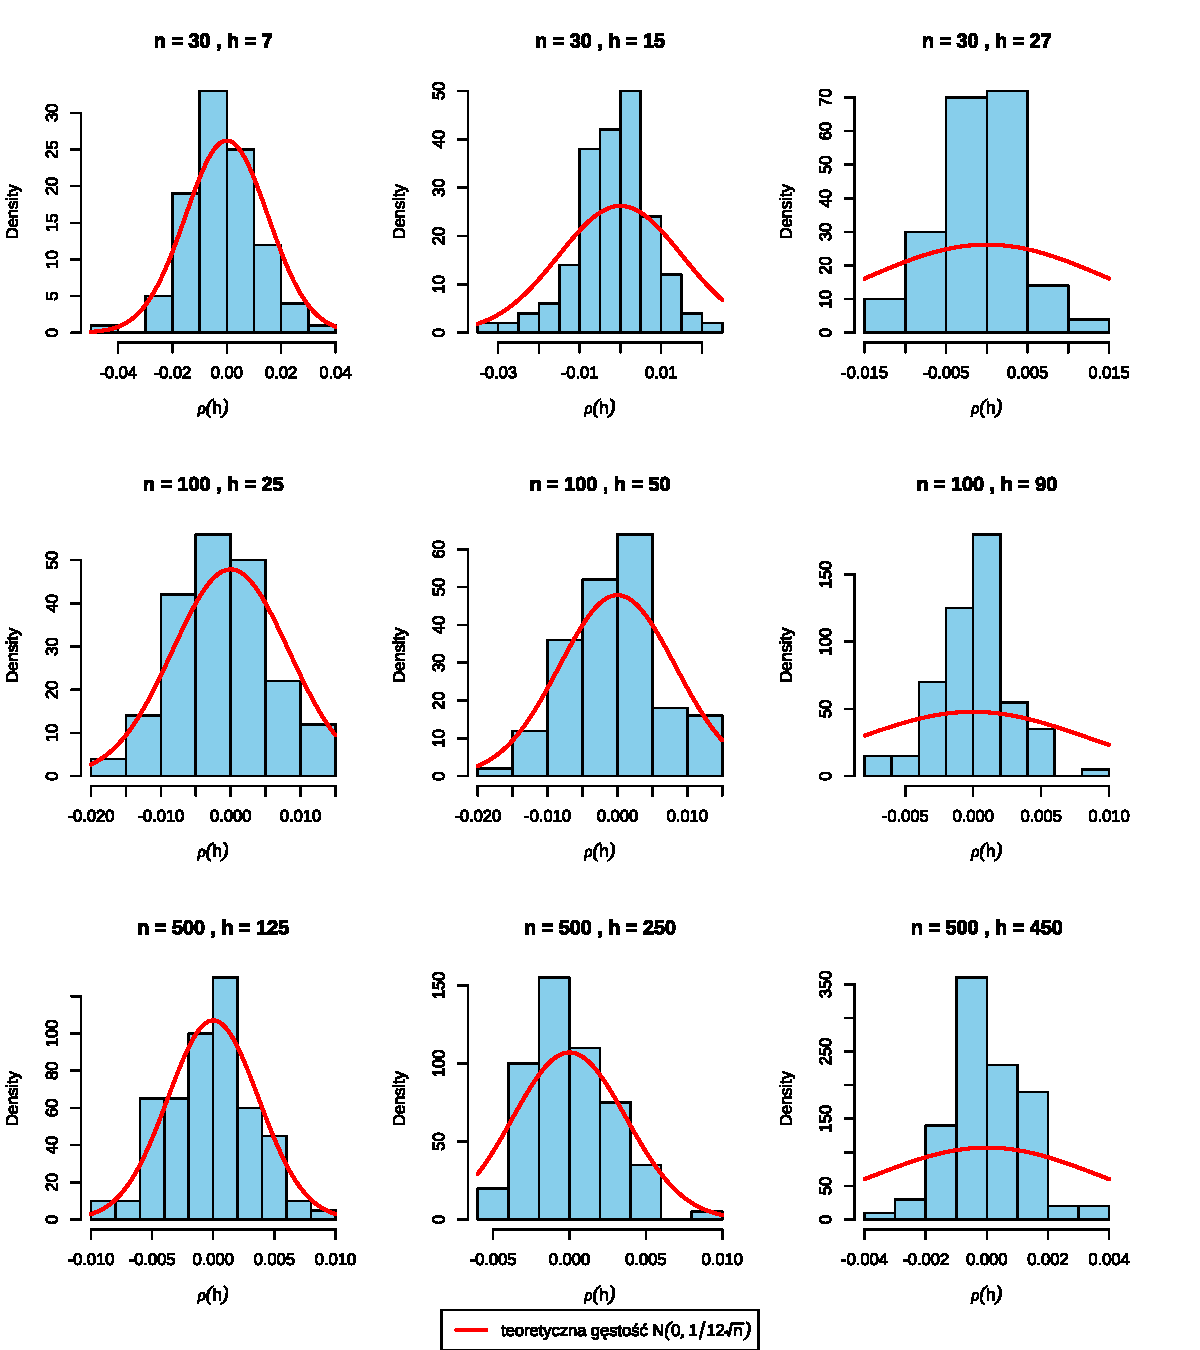
\includegraphics[width=\maxwidth]{figure/wykresy-gamma-unif-1} 

}

\caption[Histogramy dla estymatora funkcji autokowariancji dla różnych długości szeregów $n$ i różnych opóźnień $h$ z rozkładu jednostajnego]{Histogramy dla estymatora funkcji autokowariancji dla różnych długości szeregów $n$ i różnych opóźnień $h$ z rozkładu jednostajnego}\label{fig:wykresy-gamma-unif}
\end{figure}

\end{knitrout}

Wyniki dla różnych \( n \) i opóźnień \( h \) przedstawiono na [\ref{fig:wykresy-gamma-unif}]. Analiza estymatora funkcji autokowariancji dla danych z rozkładu jednostajnego wykazała następujące własności:
\begin{itemize}
    \item Dla \( n = 30 \) widoczna jest pewna asymetria rozkładu estymatora \( \hat{\gamma}(h) \), co sugeruje, że dla małych próbek rozkład nie jest jeszcze w pełni normalny
    \item Dla \( h \approx 0.9n \) histogramy wykazują większą zmienność i są mniej stabilne, co jest związane z mniejszą liczbą par obserwacji używanych do obliczenia estymatora
    \item Asymptotyczna normalność estymatora \( \hat{\gamma}(h) \) dla \( h \neq 0 \) jest osiągana dla większych próbek, takich jak \( n \geq 100 \), gdzie histogramy stają się bardziej symetryczne i skoncentrowane wokół zera
\end{itemize}

Estymator \( \hat{\gamma}(h) \) zachowuje własności asymptotyczne dla danych z rozkładu jednostajnego, ale dla małych próbek (\( n < 100 \)) i dużych opóźnień (\( h \) bliskich \( n \)), jego rozkład może odbiegać od normalnego. Dla większych próbek (\( n \geq 100 \)), aproksymacja jest dobra.



\subsection{Weryfikacja hipotez statystycznych o rozkładzie asymptotycznym estymatorów}

Przeprowadzimy formalne testy statystyczne w celu weryfikacji hipotezy o normalności rozkładów asymptotycznych estymatorów średniej i autokowariancji. Będziemy korzystać z testu Shapiro-Wilka.

Będziemy weryfikować hipotezę:

$H_0$: Badany rozkład jest zgodny z rozkładem normalnym

przeciwko:

$H_1$: Badany rozkład nie jest zgodny z rozkładem normalnym

Testy będziemy przeprowadzać na poziomie istotności $\alpha = 0.05$.

% latex table generated in R 4.3.2 by xtable 1.8-4 package
% Thu Apr 10 23:16:55 2025
\begin{table}[ht]
\centering
\caption{Odsetek przyjęć hipotezy o normalności rozkładu estymatora średniej} 
\label{tab:srednia_normalnosc}
\begin{tabular}{rrrl}
  \hline
 & n & procent\_przyjec\_H0 & rozkład \\ 
  \hline
1 & 30.00 & 95.50 & normalny \\ 
  2 & 100.00 & 94.40 & normalny \\ 
  3 & 500.00 & 94.70 & normalny \\ 
  4 & 30.00 & 77.70 & wykładniczy \\ 
  5 & 100.00 & 89.50 & wykładniczy \\ 
  6 & 500.00 & 93.30 & wykładniczy \\ 
  7 & 30.00 & 94.50 & jednostajny \\ 
  8 & 100.00 & 96.00 & jednostajny \\ 
  9 & 500.00 & 95.40 & jednostajny \\ 
   \hline
\end{tabular}
\end{table}
% latex table generated in R 4.3.2 by xtable 1.8-4 package
% Thu Apr 10 23:16:55 2025
\begin{table}[ht]
\centering
\caption{Odsetek przyjęć hipotezy o normalności rozkładu estymatora autokowariancji} 
\label{tab:autokow_normalnosc}
\begin{tabular}{rrrrl}
  \hline
 & n & h & procent\_przyjec\_H0 & rozkład \\ 
  \hline
1 & 30.00 & 1.00 & 83.00 & normalny \\ 
  2 & 30.00 & 7.00 & 82.70 & normalny \\ 
  3 & 30.00 & 15.00 & 88.40 & normalny \\ 
  4 & 100.00 & 1.00 & 93.50 & normalny \\ 
  5 & 100.00 & 25.00 & 91.60 & normalny \\ 
  6 & 100.00 & 50.00 & 94.70 & normalny \\ 
  7 & 500.00 & 1.00 & 94.40 & normalny \\ 
  8 & 500.00 & 125.00 & 94.70 & normalny \\ 
  9 & 500.00 & 250.00 & 94.80 & normalny \\ 
  10 & 30.00 & 1.00 & 34.00 & wykładniczy \\ 
  11 & 30.00 & 7.00 & 29.10 & wykładniczy \\ 
  12 & 30.00 & 15.00 & 28.80 & wykładniczy \\ 
  13 & 100.00 & 1.00 & 69.10 & wykładniczy \\ 
  14 & 100.00 & 25.00 & 64.20 & wykładniczy \\ 
  15 & 100.00 & 50.00 & 58.80 & wykładniczy \\ 
  16 & 500.00 & 1.00 & 87.70 & wykładniczy \\ 
  17 & 500.00 & 125.00 & 85.70 & wykładniczy \\ 
  18 & 500.00 & 250.00 & 85.30 & wykładniczy \\ 
  19 & 30.00 & 1.00 & 93.20 & jednostajny \\ 
  20 & 30.00 & 7.00 & 92.70 & jednostajny \\ 
  21 & 30.00 & 15.00 & 94.70 & jednostajny \\ 
  22 & 100.00 & 1.00 & 94.40 & jednostajny \\ 
  23 & 100.00 & 25.00 & 94.00 & jednostajny \\ 
  24 & 100.00 & 50.00 & 95.50 & jednostajny \\ 
  25 & 500.00 & 1.00 & 95.90 & jednostajny \\ 
  26 & 500.00 & 125.00 & 95.90 & jednostajny \\ 
  27 & 500.00 & 250.00 & 95.80 & jednostajny \\ 
   \hline
\end{tabular}
\end{table}


\newpage
Na podstawie wyników przeprowadzonych testów statystycznych (tabela \ref{tab:srednia_normalnosc} i tabela \ref{tab:autokow_normalnosc}) można sformułować następujące wnioski:

\begin{enumerate}
  \item Dla estymatora średniej (tabela \ref{tab:srednia_normalnosc}):
  \begin{itemize}
    \item W przypadku danych z rozkładu normalnego odsetek przyjęć hipotezy o normalności jest bliski 95\% dla wszystkich badanych długości szeregu, co potwierdza teoretyczne własności rozkładu tego estymatora
    \item Dla rozkładu wykładniczego, zgodność z rozkładem normalnym znacząco poprawia się wraz ze wzrostem $n$, co jest zgodne z centralnym twierdzeniem granicznym
    \item Dla rozkładu jednostajnego, nawet przy małych wartościach $n$ rozkład średniej jest bliski normalnemu
  \end{itemize}
  
  \item Dla estymatora autokowariancji (tabela \ref{tab:autokow_normalnosc}):
  \begin{itemize}
    \item Przy małych opóźnieniach ($h$) rozkład estymatora zbliża się do normalnego wraz ze wzrostem $n$ dla wszystkich badanych rozkładów
    \item Przy większych opóźnieniach (np. $h = 0.5n$) zgodność z rozkładem normalnym jest gorsza, co potwierdza obserwacje z poprzednich analiz
  \end{itemize}
  
\end{enumerate}

Wyniki te, potwierdzają teoretyczne przewidywania dotyczące asymptotycznych rozkładów badanych estymatorów i wskazują, że dla odpowiednio dużych prób ($n \geq 100$) rozkład normalny stanowi dobre przybliżenie, niezależnie od rozkładu wejściowego.

\newpage
\section{Testowanie białoszumowości}
W tym rozdziale zajmiemy się testowaniem białoszumowości dla różnych szeregów czasowych za pomocą funkcji autokorelacji. Wypróbujemy 2 podejścia - test graficzny oraz testy formalne. Wpierw zaimplementujemy test graficzny. Jako poziom istotności w naszej analizie przyjmiemy $\alpha=0.05$.
\subsection{Test graficzny} \label{sekcja1}
Do zaimplementowania graficznego testu wykorzystamy własną funkcję. Aby ten test zidentyfikował nam szereg jako biały szum, musi spełnić 2 kryteria:
\begin{enumerate}
\item Co najmniej 95\% autokorelacji próbkowych musi znajdować się w przedziale $[\frac{-1.96}{\sqrt{n}}; \frac{1.96}{\sqrt{n}}]$, gdzie ograniczenie górne podanych wartości jest kwantylem rzędu 0.975 ($1-\frac{\alpha}{2}$) rozkładu N(0,1) podzieloną przez pierwiastek z liczności próby, czyli $n$.
\item Nie ma żadnych autokorelacji próbkowych wychodzących istotnie poza przedział ufności. U nas "istotnie" będzie znaczyło, że autokorelacje próbkowe nie są większe niż $1.2\cdot\frac{1.96}{\sqrt{n}}$ i nie są mniejsze niż $1.2\cdot\frac{-1.96}{\sqrt{n}}$.
\end{enumerate}

Mając zaimplementowany test graficzny możemy sprawdzić, jak wypada test graficzny dla szumu IID z rozkładu $N(0,1)$. Jako rozmiar próby przyjmiemy $n=100$ dla większej dokładności.
\begin{figure}[H]
\begin{knitrout}
\definecolor{shadecolor}{rgb}{0.969, 0.969, 0.969}\color{fgcolor}\begin{kframe}
\begin{verbatim}
## [1] "Procent autokorelacji, które nie odstają poza przedział ufności: 1.01 %"
## [1] "Czy są istotnie odstające autokorelacje: Nie"
## [1] "Wg testu graficznego to jest biały szum"
\end{verbatim}
\end{kframe}

{\centering \includegraphics[width=\maxwidth]{figure/testowanie_białoszumowsci2-1} 

}


\end{knitrout}
\caption{Wykres autokorelacji dla szumu IID ze standardowego rozkładu normalnego}
\label{graph1}
\end{figure}

Test graficzny poprawnie rozpoznał szum IID z rozkładu normalnego jako biały szum. Na wykresie \ref{graph1} widać, że żadne wartości nie odstają poza ustalony przedział ufności. Aby mieć pewność, że jest to faktycznie szum IID wykonamy test graficzny 1000 razy na różnych próbach.
\begin{knitrout}
\definecolor{shadecolor}{rgb}{0.969, 0.969, 0.969}\color{fgcolor}\begin{kframe}
\begin{verbatim}
## Odsetek testów wskazujących, że szum IID z rozkładu N(0,1)
## jest białym szumem: 0.721
\end{verbatim}
\end{kframe}
\end{knitrout}
Test w większości przypadków rozpoznał szum IID ze standardowego rozkładu normalnego jako biały szum. Możemy wykorzystać ten test dla innych szeregów czasowych.
\begin{enumerate}
\item \label{1} \textbf{Model ruchomej średniej rzędu 1} \\
Przypomnijmy, że proces ruchomej średniej jest dany wzorem:
$$X_t=Z_t+\theta Z_{t-1},$$
gdzie $Z_t\sim WN(0,~\sigma^2$). W tym modelu przyjmiemy $\theta=0.1$.
\begin{figure}[H]
\begin{knitrout}
\definecolor{shadecolor}{rgb}{0.969, 0.969, 0.969}\color{fgcolor}\begin{kframe}
\begin{verbatim}
## [1] "Procent autokorelacji, które nie odstają poza przedział ufności: 4.04 %"
## [1] "Czy są istotnie odstające autokorelacje: Tak"
## [1] "Wg testu graficznego to nie jest biały szum"
\end{verbatim}
\end{kframe}

{\centering \includegraphics[width=\maxwidth]{figure/testowanie_białoszumowsci4-1} 

}


\end{knitrout}
\caption{Wykres autokorelacji modelu ruchomej średniej rzędu 1}
\label{graph2}
\end{figure}
W tej próbie wyszło nam, że to nie jest biały szum, jednak wynik jednej próby nie ma większego sensu ze względu na losowość. Na \ref{graph2} dokładnie widać, że co najmniej jedna autokorelacja istotnie odstaje poza przedział ufności. Aby dokładniej sprawdzić, czy nasz szereg jest białym szumem powtórzymy nasz test 1000 razy, tak jak w przypadku szumu IID z rozkładu $N(0,1)$.
\begin{knitrout}
\definecolor{shadecolor}{rgb}{0.969, 0.969, 0.969}\color{fgcolor}\begin{kframe}
\begin{verbatim}
## Odsetek testów wskazujących, że model ruchomej średniej rzędu 1
## jest białym szumem: 0.678
\end{verbatim}
\end{kframe}
\end{knitrout}

Widzimy, że w większości przypadków mamy do czynienia z białym szumem, ale potrzebne będą formalne testy, żeby jednoznacznie stwierdzić, czy faktycznie tak jest.
\item \textbf{Odwzorowanie logistyczne} \\
Zajmiemy się teraz innym przykładem - równaniem logistycznym. Przypomnijmy, że odwzorowanie logistyczne jest dane wzorem:
$$f(x)=\lambda x(1-x),~\lambda\in[0;4],~x\in[0;1].$$
W naszym przypadku niech $\lambda=1.5$.
\begin{figure}[H]
\begin{knitrout}
\definecolor{shadecolor}{rgb}{0.969, 0.969, 0.969}\color{fgcolor}\begin{kframe}
\begin{verbatim}
## [1] "Procent autokorelacji, które nie odstają poza przedział ufności: 0 %"
## [1] "Czy są istotnie odstające autokorelacje: Nie"
## [1] "Wg testu graficznego to jest biały szum"
\end{verbatim}
\end{kframe}

{\centering \includegraphics[width=\maxwidth]{figure/testowanie_białoszumowsci6-1} 

}


\end{knitrout}
\caption{Wykres autokorelacji równania logistycznego}
\label{graph3}
\end{figure}
W pojedynczej próbie wyszło nam, że jest to biały szum. Na \ref{graph3} nie ma żadnych autokorelacji odstających poza ustalony przedział ufności. Dla pewności powtórzymy test 1000 razy tak, jak w przypadku \ref{1}.
\begin{knitrout}
\definecolor{shadecolor}{rgb}{0.969, 0.969, 0.969}\color{fgcolor}\begin{kframe}
\begin{verbatim}
## Odsetek testów wskazujących, że równanie logistyczne
## jest białym szumem: 0.728
\end{verbatim}
\end{kframe}
\end{knitrout}
W tym wypadku wyszło nam, że trochę większy odsetek prób jest białym szumem niż w przypadku modelu ruchomej średniej rzędu 1. W testach formalnych dokładniej sprawdzimy, czy równanie logistyczne jest faktycznie białym szumem.
\end{enumerate}
\subsection{Testy formalne} 
\def\lf{\left\lfloor}   
\def\rf{\right\rfloor}
Zajmiemy się teraz formalnymi testami białoszumowości - testem Boxa-Pierce'a i Ljungi-Boxa. Przypomnijmy, że statystyki testowe dla obu testów prezentują się następująco:\\
\\
Dla Boxa-Pierce'a:
$$Q_{BP}=n\sum_{j=1}^h\hat\rho^2(j),$$
Dla Ljungi-Boxa:
$$Q_{LB}=n(n+2)\sum_{j=1}^h\frac{\hat\rho^2(j)}{n-j},$$
gdzie $h$ oznacza pewne maksymalne opóźnienie, a $\hat\rho(j)$ to próbkowa autokorelacja dla opóźnienia $j$. Przy założeniu, że hipoteza zerowa o białoszumowości jest prawdziwa obie statystyki mają w przybliżeniu rozkład chi-kwadrat z $h$ stopniami swobody. \\
Najpierw porównamy skuteczność obu testów przy testowaniu szumu IID z rozkładu $N(0,1)$. Z wykładu wiemy, że test Ljungi-Boxa ma lepsze własności teoretyczne, więc przeprowadzimy symulacje, aby sprawdzić, czy faktycznie daje lepsze wyniki. Oba testy są zaimplementowane w R za pomocą funkcji \verb+Box.test+, w której ustawiamy parametr $type$ odpowiednio na \verb+'Box-Pierce'+ lub na \verb+'Ljung-Box'+. Przyjmujemy $h=\lf\frac{n}{4}\rf$.
\begin{knitrout}
\definecolor{shadecolor}{rgb}{0.969, 0.969, 0.969}\color{fgcolor}\begin{kframe}
\begin{verbatim}
## W 96.6 % przypadków test Boxa-Pierce'a przyjął hipotezę o białoszumowości,
## a test Ljungi-Boxa w 91 % przypadków.
\end{verbatim}
\end{kframe}
\end{knitrout}
Co ciekawe, test Ljungi-Boxa częściej odrzucał białoszumowość szumu IID ze standardowego rozkładu normalnego. Sprawdźmy, czy tak samo będzie dla szumu z rozkładu wykładniczego z parametrem $\lambda=1$.
\begin{knitrout}
\definecolor{shadecolor}{rgb}{0.969, 0.969, 0.969}\color{fgcolor}\begin{kframe}
\begin{verbatim}
## W 97.9 % przypadków test Boxa-Pierce'a przyjął hipotezę o białoszumowości,
## a test Ljungi-Boxa w 92.8 % przypadków.
\end{verbatim}
\end{kframe}
\end{knitrout}
W tym wypadku również test Boxa-Pierce'a częściej przyjmował hipotezę o białoszumowości. Może to wynikać z tego, że wartości statystyki testu Ljungi-Boxa są bliższe rzeczywistemu rozkładowi dla skończonych prób, zatem rzadziej będzie fałszywie przyjmował hipotezę zerową niż test Boxa-Pierce'a. Oba testy jednak o wiele częściej w obu przypadkach mówiły nam, że nie mamy podstaw do odrzucenia hipotezy o białoszumowości. \\
Sprawdzimy za pomocą obu testów, czy szeregi analizowane w \ref{sekcja1} są białymi szumami.
\begin{enumerate}
\item \textbf{Model ruchomej średniej rzędu 1 (MA(1))} \label{item1}\\
Przypomnijmy, że parametr $\theta$ w tym szeregu u nas wynosi 0.1.

\begin{knitrout}
\definecolor{shadecolor}{rgb}{0.969, 0.969, 0.969}\color{fgcolor}\begin{kframe}
\begin{verbatim}
## W 95.8 % przypadków test Boxa-Pierce'a przyjął hipotezę 
## o białoszumowości, a test Ljungi-Boxa w 89.5 % przypadków.
\end{verbatim}
\end{kframe}
\end{knitrout}
Widzimy, że w tym wypadku na podstawie obu testów rozpoznajemy MA(1) z parametrem $\theta=0.1$ jako biały szum. Zobaczmy, czy dla innego parametru $\theta$, np. $\theta=0.5$, testy również powiedzą nam, że MA(1) jest białym szumem.
\begin{knitrout}
\definecolor{shadecolor}{rgb}{0.969, 0.969, 0.969}\color{fgcolor}\begin{kframe}
\begin{verbatim}
## W 44.4 % przypadków test Boxa-Pierce'a przyjął hipotezę 
## o białoszumowości, a test Ljungi-Boxa w 28.3 % przypadków.
\end{verbatim}
\end{kframe}
\end{knitrout}
Na podstawie wyników obu testów widzimy zatem, że dla innego parametru $\theta$ model ruchomej średniej rzędu 1 nie jest białym szumem. Test graficzny w tym przypadku również daje taki rezultat:
\begin{knitrout}
\definecolor{shadecolor}{rgb}{0.969, 0.969, 0.969}\color{fgcolor}\begin{kframe}
\begin{verbatim}
## Odsetek testów wskazujących, że model ruchomej średniej rzędu 1
## jest białym szumem: 0.015
\end{verbatim}
\end{kframe}
\end{knitrout}
Możemy też zmienić ilość próbek na $n=50$. Wtedy dla testów formalnych:
\begin{itemize}
\item $\theta=0.1$
\begin{knitrout}
\definecolor{shadecolor}{rgb}{0.969, 0.969, 0.969}\color{fgcolor}\begin{kframe}
\begin{verbatim}
## W 98.1 % przypadków test Boxa-Pierce'a przyjął hipotezę 
## o białoszumowości, a test Ljungi-Boxa w 88.6 % przypadków.
\end{verbatim}
\end{kframe}
\end{knitrout}
Widzimy, że w tym przypadku oba testy zgodnie w większości przypadków uznają szereg MA(1) z $\theta=0.1$ jako biały szum.
\item $\theta=0.5$
\begin{knitrout}
\definecolor{shadecolor}{rgb}{0.969, 0.969, 0.969}\color{fgcolor}\begin{kframe}
\begin{verbatim}
## W 82.1 % przypadków test Boxa-Pierce'a przyjął hipotezę 
## o białoszumowości, a test Ljungi-Boxa w 56.7 % przypadków.
\end{verbatim}
\end{kframe}
\end{knitrout}
W tym wypadku oba testy zwracają kompletnie rozbieżne rezultaty, ale oba w większości przypadków nie widzą podstaw do odrzucenia hipotezy o białoszumowści modelu MA(1) z $\theta=0.5$. Oczywiście, nie przyjmujemy tych rezultatów za prawdziwe, gdyż wiemy, że dla większego (czyli "lepszego") $n$ odrzucamy hipotezę o białoszumowości.
\end{itemize}
Dla testu graficznego:
\begin{itemize}
\item $\theta=0.1$
\begin{knitrout}
\definecolor{shadecolor}{rgb}{0.969, 0.969, 0.969}\color{fgcolor}\begin{kframe}
\begin{verbatim}
## Odsetek testów wskazujących, że model ruchomej średniej rzędu 1
## jest białym szumem: 0.849
\end{verbatim}
\end{kframe}
\end{knitrout}
Tak samo, jak wcześniej test graficzny przyjmuje hipotezę o białoszumowości szeregu MA(1) z $\theta=0.1$.
\item $\theta=0.5$
\begin{knitrout}
\definecolor{shadecolor}{rgb}{0.969, 0.969, 0.969}\color{fgcolor}\begin{kframe}
\begin{verbatim}
## Odsetek testów wskazujących, że model ruchomej średniej rzędu 1
## jest białym szumem: 0.297
\end{verbatim}
\end{kframe}
\end{knitrout}
Dla $\theta=0.5$ test graficzny odrzuca hipotezę o białoszumowości tak samo, jak wcześniej.
\end{itemize}
Biorąc pod uwagę naszą analizę dochodzimy do następujących wniosków:
\begin{wn}{Model ruchomej średniej rzędu 1 z parametrem $\theta=0.1$ jest białym szumem.} \end{wn}
\begin{wn}{Model ruchomej średniej rzędu 1 z parametrem $\theta=0.5$ nie jest białym szumem.} \end{wn}
\item \textbf{Równanie logistyczne}\\
Przypomnijmy, że parametr $\lambda$ w tym odwzorowaniu u nas wynosi 1.5.
\begin{knitrout}
\definecolor{shadecolor}{rgb}{0.969, 0.969, 0.969}\color{fgcolor}\begin{kframe}
\begin{verbatim}
## W 96.2 % przypadków test Boxa-Pierce'a przyjął hipotezę 
## o białoszumowości, a test Ljungi-Boxa w 90.3 % przypadków.
\end{verbatim}
\end{kframe}
\end{knitrout}
Widzimy, że oba testy w tym przypadku nie widzą podstaw do odrzucenia hipotezy o białoszumowości. Tak samo jak w \ref{item1}, sprawdzimy inny parametr $\lambda$, np. $\lambda=3.7$, aby zobaczyć, czy również w tym przypadku mamy do czynienia z białym szumem:
\begin{knitrout}
\definecolor{shadecolor}{rgb}{0.969, 0.969, 0.969}\color{fgcolor}\begin{kframe}
\begin{verbatim}
## W 96.2 % przypadków test Boxa-Pierce'a przyjął hipotezę 
## o białoszumowości, a test Ljungi-Boxa w 91.2 % przypadków.
\end{verbatim}
\end{kframe}
\end{knitrout}
W tym przypadku oba testy również jednogłośnie nie miały podstaw do odrzucenia hipotezy o białoszumowości. Test graficzny w tym wypadku również się zgadza z wynikami testów Boxa-Pierce'a i Ljungi-Boxa:
\begin{knitrout}
\definecolor{shadecolor}{rgb}{0.969, 0.969, 0.969}\color{fgcolor}\begin{kframe}
\begin{verbatim}
## Odsetek testów wskazujących, że równanie logistyczne
## jest białym szumem: 0.704
\end{verbatim}
\end{kframe}
\end{knitrout}
Możemy zobaczyć, czy dla $n=50$ obie formy testowania również dadzą ten sam rezultat. Dla testów formalnych:
\begin{itemize}
\item $\lambda=1.5$
\begin{knitrout}
\definecolor{shadecolor}{rgb}{0.969, 0.969, 0.969}\color{fgcolor}\begin{kframe}
\begin{verbatim}
## W 98.2 % przypadków test Boxa-Pierce'a przyjął hipotezę 
## o białoszumowości, a test Ljungi-Boxa w 89.4 % przypadków.
\end{verbatim}
\end{kframe}
\end{knitrout}
Widzimy, że dwukrotne zmniejszenie próby nie zmieniło ostatecznego rezultatu testów. Biorąc pod uwagę same testy formalne, możemy zatem przyjąć, że mamy do czynienia z białym szumem.
\item $\lambda=3.7$
\begin{knitrout}
\definecolor{shadecolor}{rgb}{0.969, 0.969, 0.969}\color{fgcolor}\begin{kframe}
\begin{verbatim}
## W 98.1 % przypadków test Boxa-Pierce'a przyjął hipotezę 
## o białoszumowości, a test Ljungi-Boxa w 90 % przypadków.
\end{verbatim}
\end{kframe}
\end{knitrout}
Dla $\lambda=3.7$ oba testy także mówią nam, że nie ma podstaw do odrzucenia hipotezy o białoszumowości. Na podstawie testów formalnych stwierdzamy zatem, że mamy do czynienia z białym szumem.
\end{itemize}
Dla testu graficznego:
\begin{itemize}
\item $\lambda=1.5$
\begin{knitrout}
\definecolor{shadecolor}{rgb}{0.969, 0.969, 0.969}\color{fgcolor}\begin{kframe}
\begin{verbatim}
## Odsetek testów wskazujących, że równanie logistyczne
## jest białym szumem: 0.844
\end{verbatim}
\end{kframe}
\end{knitrout}
Tak samo, jak dla $n=100$ test graficzny wskazuje nam, że równanie logistyczne z $\lambda=1.5$ jest białym szumem.
\item $\lambda=3.7$
\begin{knitrout}
\definecolor{shadecolor}{rgb}{0.969, 0.969, 0.969}\color{fgcolor}\begin{kframe}
\begin{verbatim}
## Odsetek testów wskazujących, że równanie logistyczne
## jest białym szumem: 0.872
\end{verbatim}
\end{kframe}
\end{knitrout}
W tym wypadku test graficzny również mówi nam, że rozważany przez nas szereg jest białym szumem.
\end{itemize}
Biorąc pod uwagę naszą analizę dochodzimy do następujących wniosków:
\begin{wn}{Równanie logstyczne z parametrem $\lambda=1.5$ jest białym szumem.} \end{wn}
\begin{wn}{Równanie logstyczne z parametrem $\lambda=3.7$ jest białym szumem.} \end{wn}
\end{enumerate}

\end{document}
